\chapter{Object Design}
\label{ch:ObjectDesign}

During object design, we refine the system design artifact of Chapter \ref{ch:SystemDesign} to detail the specifications for each subsystem. Therefore, we define the subsystem interfaces and identify off-the-shelf components that can be reused to provide the functionality of a subsystem. Furthermore, design patterns are selected to solve common problems and ensure future extensibility of the subsystems in which they are used. The subsystem decomposition model in Figure \ref{fig:subsystemDecomposition} is restructured to reflect the changes we introduced in defining the interfaces of the subsystems to improve the maintainability of our system. Finally, we detail our test strategy, which ensures that all functional and nonfunctional requirements are met. For that, we describe the inputs and expected outputs for each subsystem and type of test to be performed. 

In Section \ref{sec:Reuse}, we identify and describe off-the-shelf components and design patterns, that can be used to realize our subsystems. Since our system does not prescribe using a specific programming language, we consider multiple off-the-shelf components for each subsystem. Section \ref{sec:InterfaceSpecification} describes the specification of our subsystems' interfaces by specifying their operations and important properties. Furthermore, we define the structure of the machine-readable migration guide in detail. The class diagrams reflect the design patterns used in each case. By specifying the interfaces, potential improvements of our system model are revealed. In Section \ref{sec:Restructuring} all modifications are explained and the updated diagram of our subsystem decomposition is provided. Section \ref{sec:Testing} outlines our test strategy and details the tests to be performed as well as their corresponding inputs and expected outcomes. While our unit tests are designed to detect faults of individual subsystems and components, our integration tests define an appropriate interaction of multiple components. Our system tests are derived from the functional requirements and are used to validate the functionality of the overall system.

The resulting object design model can be divided into modules that can be implemented by individual developers. It provides the foundation for an instantiation of our system, which is described and used in Chapter \ref{ch:CaseStudyEvaluation} to evaluate our approach.

\newpage
\section{Reuse}
\label{sec:Reuse}

 Software reuse increases the productivity of development teams and improves the overall quality of the product. Therefore, our proposed system defines several components that can be reused from existing solutions. All external components must be open-sourced under the MIT license in order to fulfill our non-functional requirement \ref{nfr:Legal}. Furthermore, custom components of subsystems can be implemented by reusing pattern solutions as defined by the \ac{GoF}. 
 
 Tooling to parse an IDL specification and generate library code for various programming languages is available for many modern Web APIs. For REST-based Web APIs, the OpenAPI Generator\footnote{https://openapi-generator.tech/} is an open-source tool that can be integrated in existing Java projects via Maven/Gradle plugins, or used via CLI and an online service\footnote{http://api.openapi-generator.tech/index.html}. It supports parsing of OpenAPI IDLs regardless of whether they were encoded to YAML or JSON. Additionally, it generates library code in 65 programming languages and dialects. Google's gRPC\footnote{https://grpc.io/} technology uses protocol buffers as an IDL and as a format for exchanging messages. Parsing protocol buffers and generating library code is currently available for 16 programming languages and dialects, with support for additional languages upcoming. Emerging GraphQL\footnote{https://graphql.org/} APIs are described by the \ac{SDL} for which different tools exist that are able to generate library code from it. On the one hand, the GraphQL code generator\footnote{https://graphql-code-generator.com/} supports five programming languages and offers several configuration options to further customize the emitted code. Quicktype\footnote{https://quicktype.io/}, on the other hand, supports 19 programming languages and similar configuration options. One limitation of all tools above is their integrability as a framework. They are designed to generate library code persisted in files, which prevents developers from accessing intermediate artifacts like the decoded IDL document. Generating source code in a programming language that is not supported by those tools requires forking the codebase to extend their functionality. However, for some IDLs and programming languages new frameworks are published that can be integrated into existing projects to get access to intermediate artifacts. For example, the OpenAPIKit\footnote{https://github.com/mattpolzin/OpenAPIKit} is an open-source project that offers a Swift library to en-/decode OpenAPI IDL documents. By separating the parsing of an IDL document and the subsequent library generation, the extensibility for new programming languages and IDL types is considerably increased. 
 
 Supporting multiple programming languages is also a challenge for the \texttt{Source\-Code} \texttt{Importer} subsystem. It must support parsing source code of a programming language into its \ac{AST}. Tools are available for most programming languages as many features of \acp{IDE} like syntax highlighting or auto-completion rely on them. However, most of these tools are commercial products and are not available under an open-source licence. One example is the JavaParser\footnote{https://javaparser.org/} which is available as a Maven and Gradle plugin for parsing, analyzing and generating Java code. Other frameworks were created through the active contribution of open source communities. Acorn\footnote{https://github.com/acornjs/acorn} is a parser for JavaScript code that supports plugins for JavaScript dialects and frameworks like React JSX. Sourcery\footnote{https://github.com/krzysztofzablocki/Sourcery} is a Swift library that provides an \ac{API} that offers parsing and generating Swift code based on Stencil templates. All of these frameworks are limited to parsing source code of a single programming language. To support many different languages simultaneously, custom lexers and parsers must be specified and implemented for each language. While this is a cumbersome manual effort, tools like \ac{ANTLR}\footnote{https://www.antlr.org/} enable developers to generate lexers and parsers in Java, C\#, C++, JavaScript, Python, Swift and Go. Therefore, users have to provide a grammar of the language that describes its structure. This grammar is defined using the Antlr4 grammar syntax. The application's repository contains over 200 predefined grammars that cover many modern programming languages.
 
 Our system uses a machine-readable migration guide to collect all changes that were introduced between subsequent versions of a Web API. In order to fulfill \ref{nfr:MigGuideFormat}, it should be using a \ac{DSL} that is in a human-readable format which is prevalent in the context of web development. While an implementation in a custom language using the auxiliary features of ANTLR would be conceivable, we advocate the use of \ac{JSON} as an external, compositional DSL. This decision is based on the fact that JSON is not just easy to understand and learn, but is also an established standard that is widely adopted by web developers. Another key advantage comes from existing utility libraries for parsing JSON documents in many programming languages. As they are either part of core libraries or can be integrated using third-party open source frameworks, the need to use a custom built lexer and parser is eliminated. Listing \ref{lst:exampleGuide} shows an example JSON-based migration guide that contains one change and specifies some meta-information.
 
 \vspace{2mm}
 \begin{lstlisting}[language=json, caption={Examplatory migration guide in JSON format}, captionpos=b, label={lst:exampleGuide}]
 	{
 		"summary" : "This is an examplatory migration guide.",
 		"api-spec": "OpenAPI",
 		"from-version" : "0.0.1b",
 		"to-version" : "0.0.2",
 		"changes" : [
	 		{
	 			"reason": "Default value was added.",
	 			"object" : {
	 				"operation-id" : "findPetsByStatus",
	 				"defined-in" : "/pet"
	 			},
	 			"target" : "Content-Body",
	 			"added" : [
		 			{
		 				"name" : "_",
		 				"type" : "Pet",
		 				"default-value" : "{ 'type' : 'Cat', age: 2 }"
		 			}
	 			]
	 		}
 		]
 	}
 \end{lstlisting}
 
The decoded representation of a migration guide is used by the \texttt{Migration} \texttt{Manager} subsystem to adapt previous facade code to the changes it contains. Although there are no off-the-shelf components that can be reused, patterns have been identified that are applicaple here. The behavior of the \texttt{Migration} component depends solely on the changes in the migration guide. Therefore, an alternative computational model is to be preferred in contrast to the common imperative models, in which code is organized in an object-oriented manner \cite{fowler_domain-specific_2011}. Fowler et. al coined the term \textit{Semantic Model} to define models that are populated by a \ac{DSL}.  The authors further define an \textit{Adaptive Model} as a specific variation of a Semantic Model in that they take the primary behavioral role in a system. According to the authors, Adaptive Models enable developers to shift the execution context from compile time to runtime and thus change behavior of a running system without a recompile. As the defined behavior is implicit, their implementation is difficult to understand and maintain \cite{fowler_domain-specific_2011}. The ability to alter the migration behavior during runtime by specifying changes in an external migration guide outweighs the negative aspects of using this pattern to model the \texttt{Migration} component. 

Before the generated source code emitted by the \texttt{Library} \texttt{Generation} and \texttt{Facade} \texttt{Generation} subsystems is persisted, users are able to specify formatting rules in order to fulfill \ref{nfr:CodeStyle}. Therefore, multiple open source tools have been created for every modern programming language. SwiftFormat\footnote{https://github.com/apple/swift-format} is an open source tool that formats Swift code using a predefined ruleset. It can be used either via \ac{CLI} or by integrating its framework into an existing Swift application. Prettier\footnote{https://prettier.io/} is a code formatter for multiple languages and dialects used in web development. It supports formatting of JavaScript, JSX, TypeScript and more. Additionally, its active community provides plugins for even more languages like Java, Swift and Ruby. Prettier can be integrated in \acp{IDE} or CI environments and provides an \ac{API} to be used within JavaScript applications. 

All subsystem that deal with importing or generating different types of programming languages or IDL documents are required to adapt their behavior based on the needs of the user. User preferences are provided by configuration options and need to be applied during runtime. The \textit{Strategy} pattern \cite{gamma_design_1995} is a behavioral design pattern that enables selecting these preferences without the need to recompile the application \cite{bruegge_object-oriented_2010}. In our proposed system we identified four subsystems that benefit from applying this pattern.

As shown in Figure \ref{fig:outcome}, our system emits library code that distinguishes between different layers that serve their own purpose. The library layer issues requests and receives responses directly from the Web API. It offers an interface to the facade layer that adapt to changes within the library layer without altering its own public interface. Client applications are unaware of the internal behavior of the facade layer and the interfaces of the library layer. The \textit{Facade} pattern \cite{gamma_design_1995} used here is a software design pattern that enables masking of internal behavior and any changes made to it.
 
\section{Interface Specification}
\label{sec:InterfaceSpecification}

Reusable components and pattern used to create custom components offer their functionality via public-facing interfaces. A detailed specification of these interfaces is required to enable an integration of all subsystems. Additionally, each subsystem defines artifacts that they produce for and consume from other components. The following section demonstrates the internal structure of custom components while for reused third-party subsystems their integration and emitted artifacts are illustrated.

\begin{figure}[!h]
	\centering{
		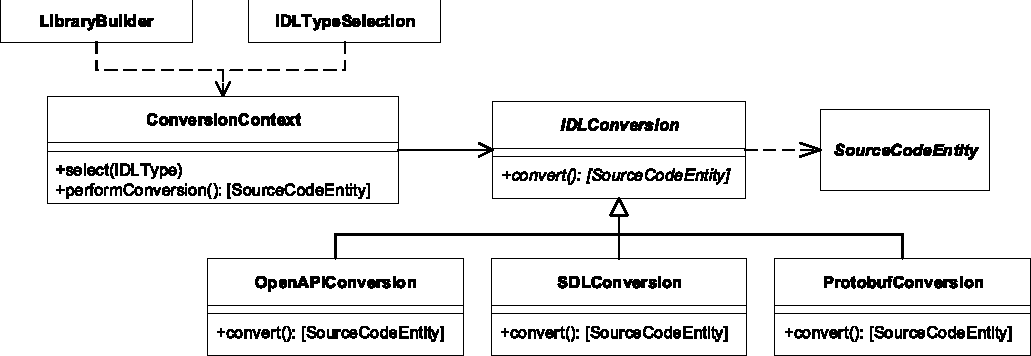
\includegraphics[width=150mm]{images/cd_idl_import.pdf}
		\caption{Class diagram of IDL importer subsystem}
		\label{fig:cdIDLImport}
	}
\end{figure}

Importing an \ac{IDL} for a specific type of Web API needs to flexibly switch between different implementations for various kinds of \acp{IDL}. Therefore, the strategy pattern is used to abstract the internal implementation from the consuming client code. The \texttt{LibraryBuilder} is the client that uses the \texttt{performConversion} method. Depending on the type of IDL which was set by the \texttt{IDL\-Type\-Selec\-tion} for the \texttt{ConversionContext}, the appropriate implementation of \texttt{IDL\-Con\-ver\-sion} performs the conversion and returns a list of \texttt{SourceCodeEntity} objects. 

\begin{figure}[!h]
	\centering{
		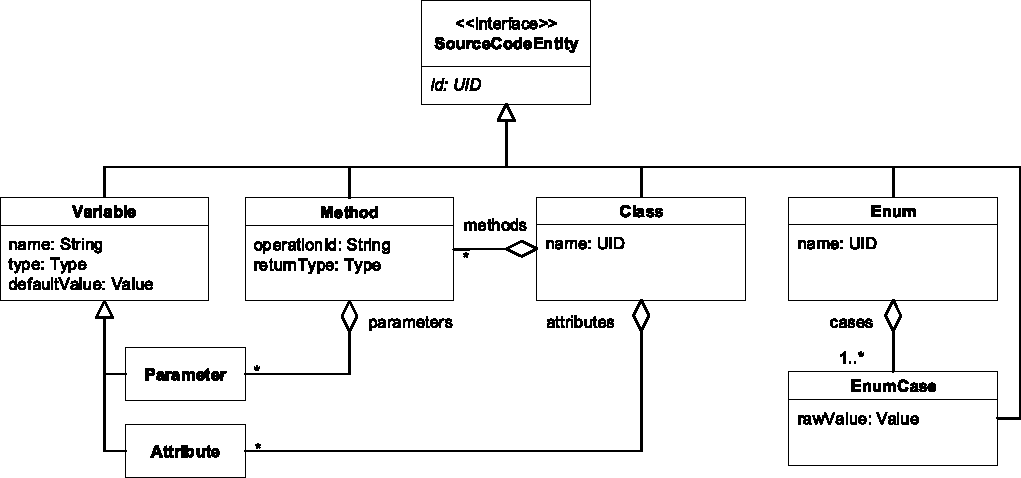
\includegraphics[width=150mm]{images/cd_sourceentity.pdf}
		\caption{Class diagram of source code entity artifact}
		\label{fig:cdSourceCodeEntity}
	}
\end{figure}

\texttt{SourceCodeEntity} objects are used by multiple components. They represent the basic syntactical elements that are common in all modern programming languages. Figure \ref{fig:cdSourceCodeEntity} shows their composition and their most important attributes and relations. \texttt{Class}, \texttt{Method} and \texttt{Enum} entities represent structual elements in which other elements can be nested. A \texttt{Class} element contains \texttt{Attributes} and \texttt{Methods}, whereas \texttt{Enums} specify at least one \texttt{EnumCases}. Each \texttt{Source\-Code\-Entity} can be identified by a \ac{UID}. For \texttt{Class} and \texttt{Enum} elements, their name itself is unique, while for \texttt{Variables}, \texttt{Methods} and \texttt{EnumCases} their context needs to be taken into account.

\begin{figure}[!h]
	\centering{
		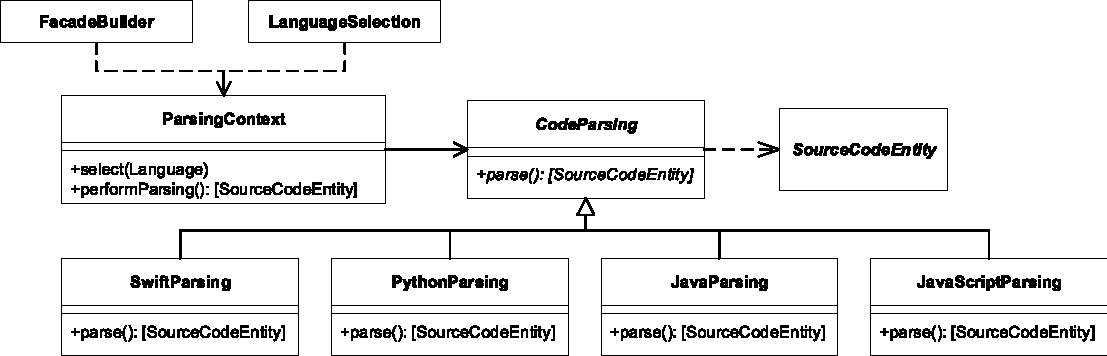
\includegraphics[width=150mm]{images/cd_code_import.pdf}
		\caption{Class diagram of code importer subsystem}
		\label{fig:cdCodeImport}
	}
\end{figure}

Adapting a previous facade to recent changes of a Web API requires importing its source code. Therefore, the \texttt{SourceCode} \texttt{Importer} subsystem must be able to parse source code of multiple programming languages. The decision which programming language needs to be parsed is made during runtime by the user. Since the requirements are the same as those for importing different types of \acp{IDL}, the strategy design pattern is also used here. The selection of the programming language to parse is done by the \texttt{Language\-Selection} component while the \texttt{Facade\-Builder} requests the parsed \texttt{Source\-Code\-Entity} objects.

\begin{figure}[!h]
	\centering{
		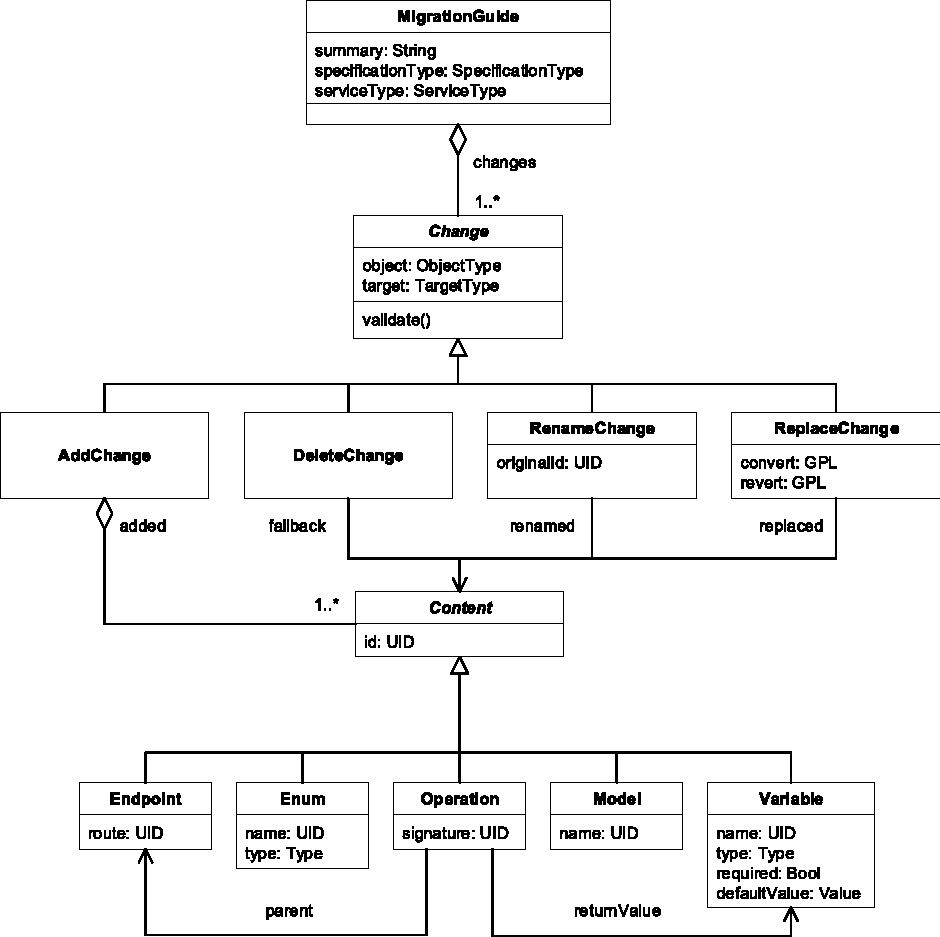
\includegraphics[width=155mm]{images/cd_migguide.pdf}
		\caption{Class diagram of migration guide artifact}
		\label{fig:cdMigrationGuideArtifcat}
	}
\end{figure}

In addition to the decoded representation of the previous facade code, the migration guide needs to be parsed, too. Based on our decision to use \ac{JSON} for defining a migration guide, it can be parsed using a language's core libraries or third-party components. The decoded migration guide structure is shown in Figure \ref{fig:cdMigrationGuideArtifcat}. 

A migration guide contains the type of \ac{IDL} specification in which the Web API is described as well as its service type. Additionally, it specifies all changes that were introduced by the latest version of the Web API. Every change is associated with one of four change types. \texttt{Add\-Changes} denote, that one or more elements of a Web API were added to it. This includes for example adding attributes to a model, parameters to a method or methods to an endpoint. \texttt{Delete\-Changes} indicate that an element was removed from the Web API. For migratable deletions such as removing an attribute of a model, a fallback value can be specified which is used instead of the removed value. \texttt{Rename\-Changes} are used to automate refactorings. Since the functionality of a renamed element remains unchanged, only the previous and new identifications have to be specified here. 

Elements that were renamed and whose functionality also changed are specified with \texttt{Replace\-Changes}. They are the most complex type of change as they need to contain not only the replacement element, but additionally instructions on how to revert them to their previous version and convert their previous to their current version. Code stated in a \texttt{Replace\-Change} needs to be converted into statements of the programming language specified by the user. Instead of introducing another \ac{DSL} or extending the migration guide \ac{DSL}, we decided to use a \ac{GPL} that is common to web developers. We chose JavaScript for that purpose, as it is one of the most used programming language by web developers and it complements \ac{JSON} well. Furthermore, JavaScript code can be directly executed by an interpreter without previously compiling it. Various programming languages support interpreting JavaScript code. For example, Microsoft provides Windows Script Engines\footnote{https://docs.microsoft.com/en-us/previous-versions/windows/internet-explorer/ie-developer/windows-scripting/windows-script-engines} for C\# and Apple released the framework JavaScriptCore\footnote{https://developer.apple.com/documentation/javascriptcore} for Swift and Objective-C in order to parse and interpret JavaScript at runtime .

Each type of change is applied to one object of the Web API and targets one property of it. For example, adding a parameter to a method results in an \texttt{Add\-Change} for a \texttt{Method} object type with a \texttt{Parameter} target type while renaming a model results in a \texttt{Rename\-Change} for a \texttt{Model} object type with a \texttt{Signature} target type. All changes reference \texttt{Content}, i.e. the unique identification of an element of the Web API including additional information that supports the migration process. Invalid changes are indicated by an incorrect combination of their internal information. They are identified by their validation method which reports any errors to the user.

\begin{figure}[!h]
	\centering{
		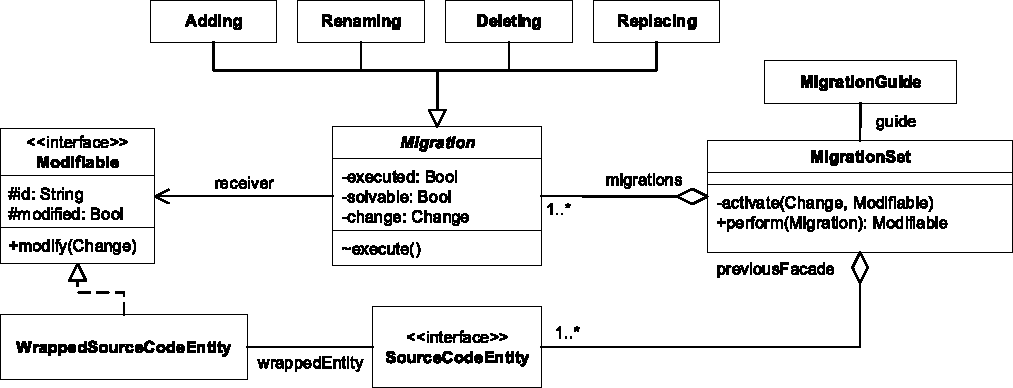
\includegraphics[width=150mm]{images/cd_migration.pdf}
		\caption{Class diagram of migration manager subsystem}
		\label{fig:cdMigrationManager}
	}
\end{figure}

For performing the migration steps, the \texttt{Migration} \texttt{Manager} subsystem incorporates the imported migration guide and decoded previous facade. Analogous to the types of changes corresponding types of migration are defined. \texttt{Migrations} contain the change that must be migrated as well as information that indicates whether they are solvable and have been executed. Furthermore, they reference a \texttt{Modifiable} object on which the migration is performed. The \texttt{Modifiable} interface is implemented by a wrapper component that acts as an adapter for modifying a \texttt{SourceCodeEntity} of the previous facade. By executing a \texttt{Migration}, the \texttt{modify} method of a \texttt{Modifiable} is triggered which adapts the \texttt{SourceCodeEntity} according to the type of migration. The \texttt{mo\-di\-fied} property of a \texttt{Modifiable} denotes that this object has already been migrated. All migrations as well as the previous facade are composed in the \texttt{MigrationSet}. By analyzing the changes stated in the migration guide and their target entities, it creates the corresponding migrations by invoking the \texttt{ac\-ti\-vate} method. Unsupported or incorrect combinations result in an unsolvable migration. The \texttt{MigrationSet} is the public interface of the subsystem by providing the \texttt{perform} method to perform a migration and return the adapted facade element.

\begin{figure}[!h]
	\centering{
		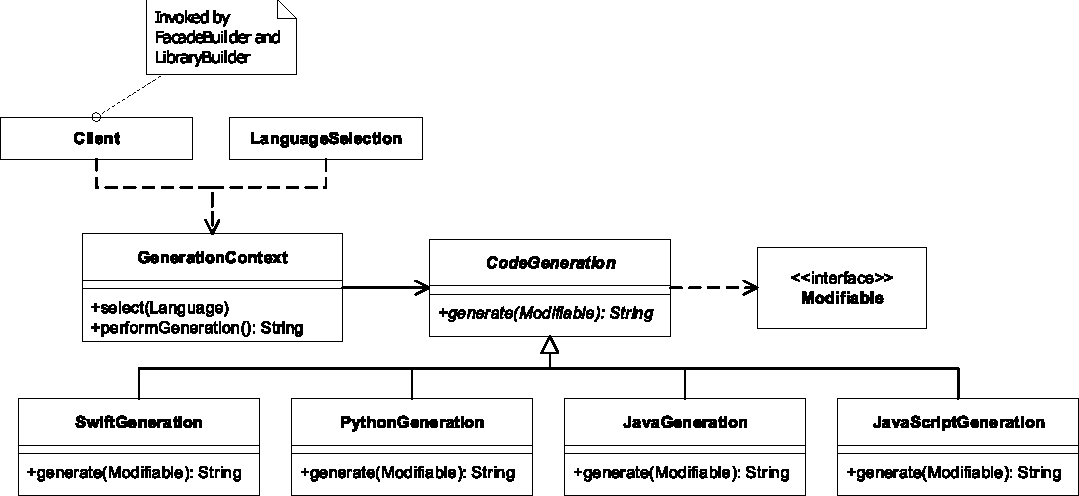
\includegraphics[width=155mm]{images/cd_generation.pdf}
		\caption{Class diagram of code generator subsystem}
		\label{fig:cdGenerator}
	}
\end{figure}

Generating source code from decoded entities for various programming languages requires the \texttt{Code} \texttt{Generator} subsystem to use the strategy pattern. Thereby, the subsystem can select the correct syntax elements during runtime. In contrast to the \texttt{SourceCode} \texttt{Importer} subsystem, it takes wrapped \texttt{SourceCodeEntity} objects as input and generates a string of compilable source code in the programming language the user specified. Its service is used by the subsystems concerned with generating the library code for an IDL and generating the migrated facade code.

\begin{figure}[!h]
	\centering{
		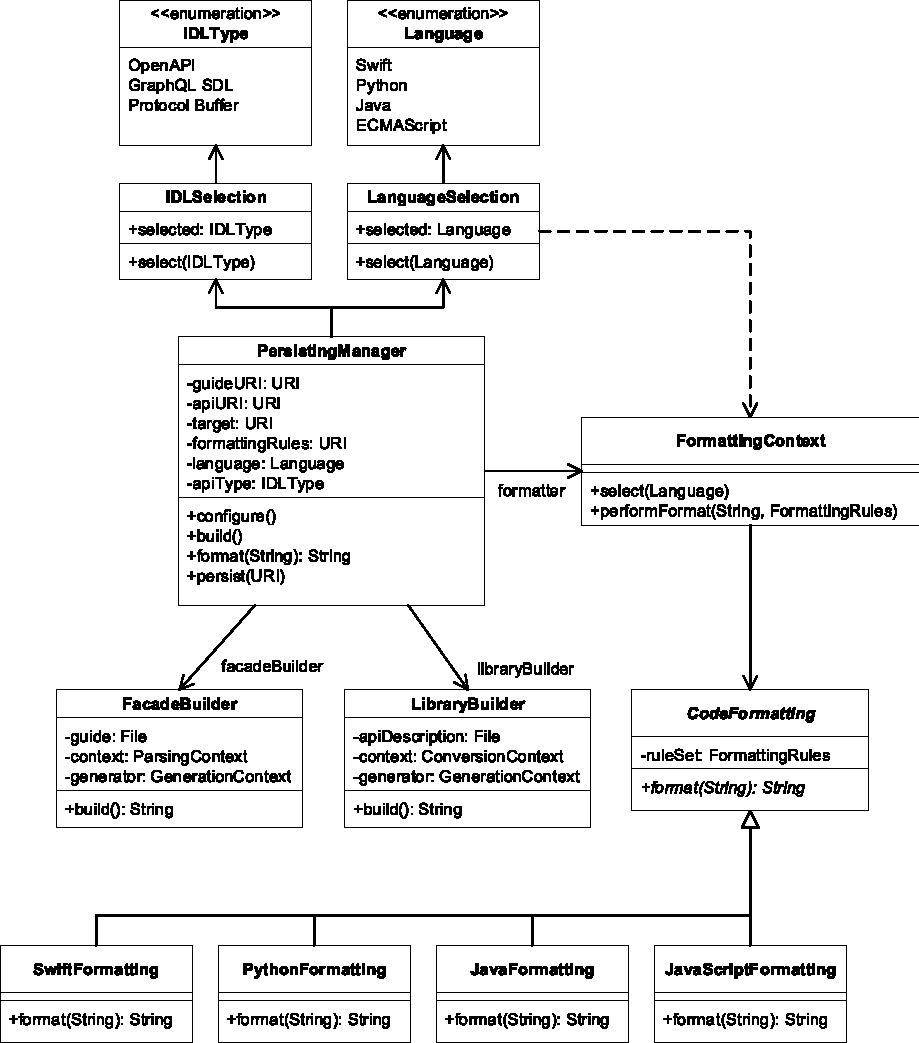
\includegraphics[width=155mm]{images/cd_persisting.pdf}
		\caption{Class diagram of persisting manager subsystem}
		\label{fig:cdPersisting}
	}
\end{figure}

The whole process is orchestrated by the \texttt{Persisting} \texttt{Manager} subsystem. The \texttt{Persisting} \texttt{Manager} takes the user input and selects the desired type of \ac{IDL} and programming language. Additionally, it contains all configuration options of the user that are necessary to retrieve the Web API's \ac{IDL} and migration guide. Furthermore, it contains the ruleset specifying the formatting style of the source code. After configuring the system according to the user's input, the \texttt{build} method starts the importing, adapting and generating process. Therefore, the \texttt{LibraryBuilder} and \texttt{FacadeBuilder} objects are instantiated and their \texttt{build} method is executed. Both objects hold references to their subsystems that are responsible for generating library code from an imported \ac{IDL} and generating source code of an adapted facade, respectively. Once it receives the generated source code strings, the \texttt{PersistingManager} formats the code using a \texttt{Code\-For\-mat\-ting} component instantiated according to the currently selected programming language. As this is done at runtime, the strategy pattern is also applied here. Formatting source code is available by using third-party components for many programming languages, e.g. SwiftFormat\footnote{https://github.com/apple/swift-format} for Swift and Prettier\footnote{https://prettier.io/} for JavaScript und Java. The formatted source code is then persisted by invoking the \texttt{persist} method. Although the internal structure of the emitted library is defined by our system, the user is able to specify its identifier and its target location.
\section{Restructuring}
\label{sec:Restructuring}

After specifying the interfaces of all components, the subsystem decomposition needs to be restructured to reflect all changes. Regarding the generation of code in various programming languages, we identified that the \texttt{Migration} \texttt{Manager} and \texttt{Library} \texttt{Generation} subsystems require the same functionality. As a result, a \texttt{Code} \texttt{Generation} subsystem was extracted that provides its service to the \texttt{Migrator} component and the \texttt{IDL} \texttt{Conversion} subsystem. By that no redundant functionality has to be implemented. 

Additionally, we decided to use JavaScript for handling convert and revert operations defined in \texttt{Replace\-Changes}. Therefore, the \texttt{Source\-Code} \texttt{Importer} subsystem must support parsing it. The restructured subsystem decomposition is illustrated in Figure \ref{fig:subsystemRestructured}.

\begin{figure}[!h]
	\centering{
		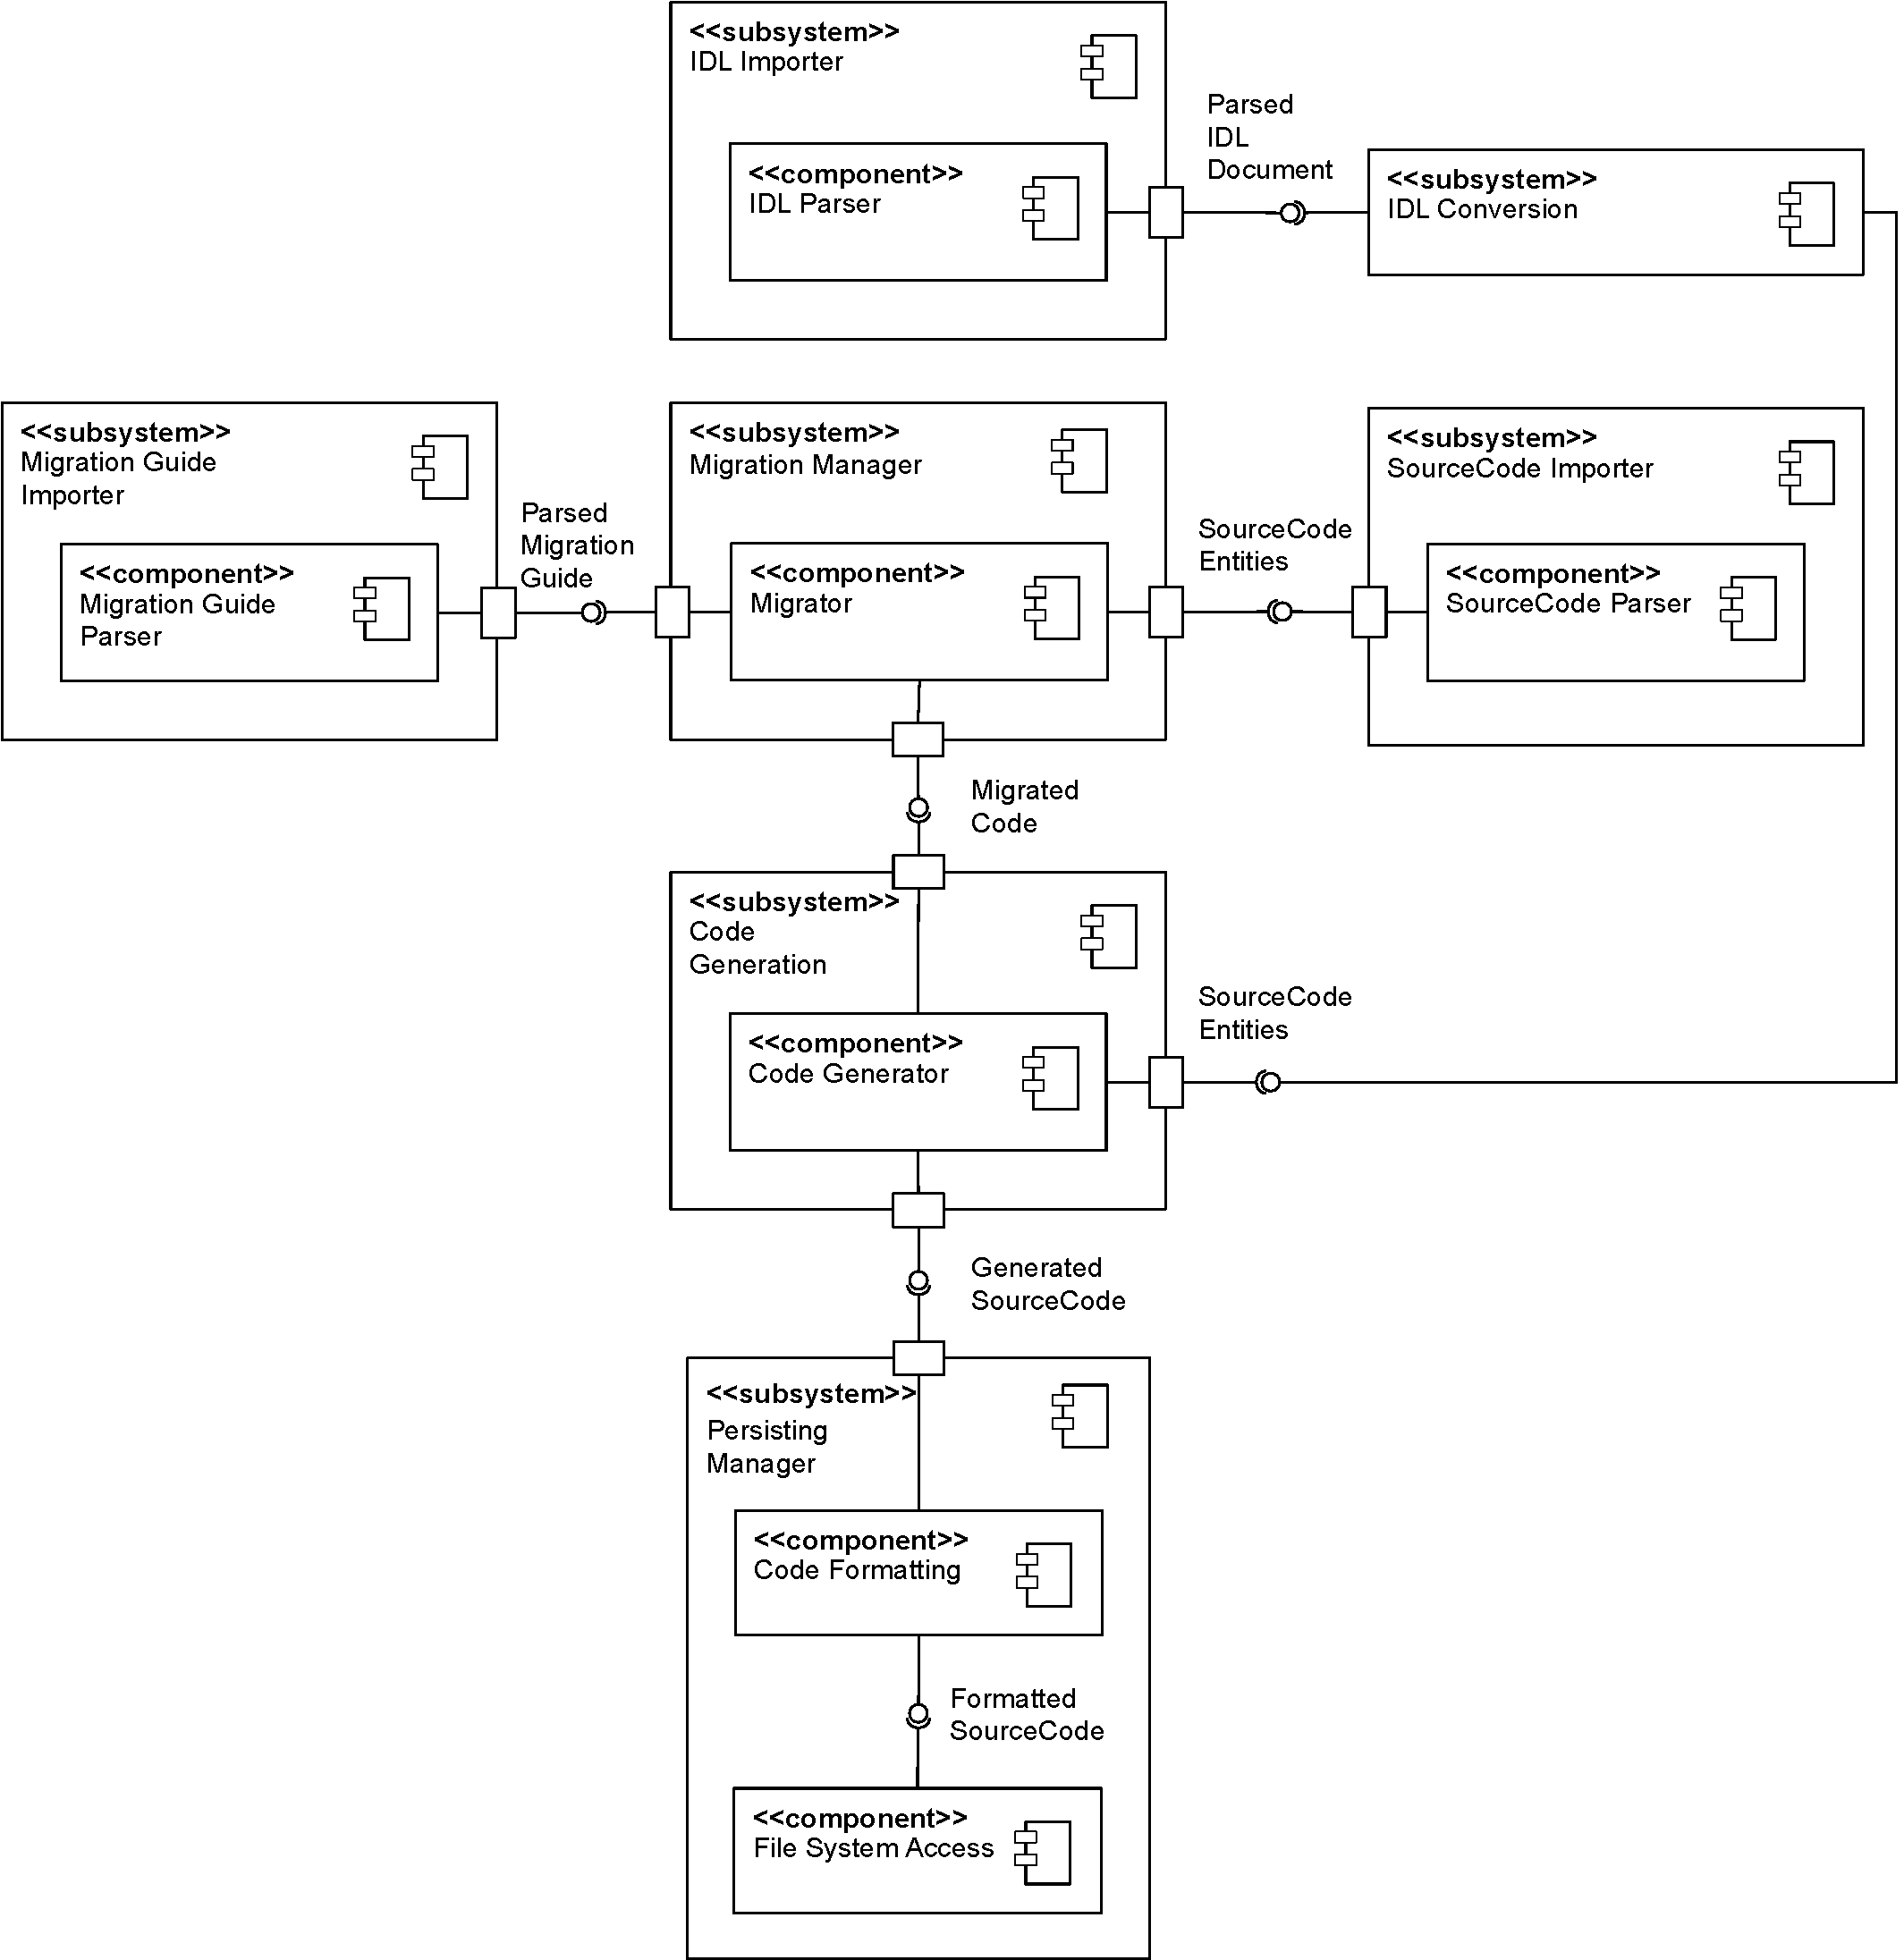
\includegraphics[width=155mm]{images/subsystem_restructured.pdf}
		\caption[Restructured subsystem decomposition]{Restructured subsystem decomposition - The \texttt{Code Generation} subsystem was extracted from the \texttt{Migration Manager} and \texttt{Library Generation} subsystems to provide a uniform interface to both subsystems}
		\label{fig:subsystemRestructured}
	}
\end{figure}
\section{Testing}
\label{sec:Testing}

Testing ensures that all requirements defined in Section \ref{sec:Requirements} and use cases detailed in Section \ref{sec:UseCases} are fulfilled. Therefore, unit tests are specified that test all components of our subsystems in isolation. Furthermore, our integration tests demonstrate the faultless interaction between our subsystems. System tests are defined to ensure that the fully integrated application produces the correct output for various inputs. The testing strategy of our proposed system is subsequently described in a structured manner according to these types of tests.

\paragraph{Unit testing} Unit tests are used to find faults in subsystems with respect to use cases from use case models \cite{bruegge_object-oriented_2010}. Any subsystem for which a custom implementation is preferred over using a third-party component requires extensive testing.

Testing \texttt{UC1}, all subsystems affected by integrating our system are tested in isolation. Various IDL documents must be used as an input for the \texttt{IDL} \texttt{Importer} subsystem which determines their validity and provides the parsed document. While correct IDL specifications are processed without interruption, invalid or incomplete IDL documents raise an error message in the component which is forwarded to the user. Test cases need to be defined for each type of IDL that is supported by the system. For testing the \texttt{IDL} \texttt{Conversion} subsystem, examplatory parsed entites of IDL documents are used to find faults in the conversion algorithm. Its expected output is manually defined and validated based on the emitted source code entities. When the system is set up for the first time, a new facade must be created without migrated changes. Hence, the \texttt{Source\-Code} \texttt{Importer} targets the generated library code in order to create source code entities. Testing this process requires examplatory source code files in various programming languages that are validated based on previously defined source code entities. Empty or invalid files raise a parsing exception. Producing the textual representation of source code needs to be validated by testing the algorithm of the \texttt{Code} \texttt{Generation} subsystem for each supported programming language. Therefore, example collections of source code entities are used as an input that are transformed into strings of source code in the respective language. The unformatted source code strings are formatted by the \texttt{Persisting} \texttt{Manager} subsystem which is tested by validating the formatted source code based on predefined examples. 

\renewcommand{\arraystretch}{1.5}
\begin{table*}[ht]
	\begin{center}
		\begin{tabular}{|>{\raggedright\arraybackslash}m{4cm}|>{\raggedright\arraybackslash}m{5cm}|>{\raggedright\arraybackslash}m{5cm}|}
			\hline
			\begin{center}
				\textbf{Subsystem/ Component}
			\end{center} &  \begin{center}
			\textbf{Input} 
		\end{center}&  \begin{center}
		\textbf{Output}
	\end{center} \\ \hline
			\textit{IDL Importer} & Invalid or incomplete IDL document & Error message \\ \hline
			\textit{IDL Importer} & Valid IDL document & Parsed IDL document \\ \hline
			\textit{IDL Conversion} & Parsed IDL document & Source code entities \\ \hline
			\textit{SourceCode Importer} & Compilable source code  files & Source code entities \\ \hline
			\textit{SourceCode Importer} & Uncompilable source code files & Error message \\ \hline
			\textit{SourceCode Importer} & Source code entities & Unformatted, compilable source code strings  \\ \hline
			\textit{Code Formatting} & Unformatted, compilable source code strings & Formatted source code strings  \\ \hline
		\end{tabular}
		\caption{Input and output of subsystem unit tests for UC1}\label{tbl:UnitTestsUC1}
	\end{center}
\end{table*}

Testing the automated migration is required to detect faults during the upgrade of client source code after the Web API changed (\texttt{UC4}). In addition to the ones defined for \texttt{UC1}, test cases need to be specified that cover importing a machine-readable migration guide and the adaption of the facade to the changes it contains. Since the migration guide is structured using \ac{JSON}, unit tests for the \texttt{Migration} \texttt{Guide} \texttt{Importer} subsystem are performed by the developers of the third-party component. Migrating a previous facade must focus all types of migrations. Additionally, test cases need to be defined for combining different types of changes targeting the same object. Testing this subsystem requires providing example migration guides and manually specified source code entities of a previous facade as an input. Validation is performed by matching the migrated source code entities to predefined end-results. By creating unsolvable \texttt{Migrations}, edge cases can be simulated that result in error messages which need to be forwarded to the user. For example, adding a new parameter to a model of the Web API is unsupported and raises an error message. The message contains information about the type of change, the target object, and a reason for the fault. Incomplete \texttt{Migrations}, i.e. \texttt{Migrations} that do not contain a change, must not be created and result in an unsolvable \texttt{Migration}.

\begin{table*}[ht]
	\begin{center}
		\begin{tabular}{|>{\raggedright\arraybackslash}m{4cm}|>{\raggedright\arraybackslash}m{5cm}|>{\raggedright\arraybackslash}m{5cm}|}
			\hline
			\begin{center}
				\textbf{Subsystem/ Component}
			\end{center} &  \begin{center}
				\textbf{Input} 
			\end{center}&  \begin{center}
				\textbf{Output}
			\end{center} \\ \hline
			\multirow{2}{*}{\textit{Migration Manager}} & Parsed migration guide with changes of multiple target objects & \multirow{2}{5cm}{Migrated source code entities}  \\
			& Source code entities &  \\ \hline
						\multirow{2}{*}{\textit{Migration Manager}} & Parsed migration guide with multiple changes of a single target object & \multirow{2}{5cm}{Migrated source code entities}  \\
			& Source code entities &  \\ \hline
						\multirow{2}{*}{\textit{Migration Manager}} & Parsed migration guide with invalid changes & \multirow{2}{5cm}{Unsolvable Migration object}  \\
			& Source code entities &  \\ \hline
		\end{tabular}
		\caption{Additional input and output of subsystem unit tests for UC4}\label{tbl:UnitTestsUC4}
	\end{center}
\end{table*}

\paragraph{Integration testing} The subsequent tests are used to find faults by testing individual components in combination \cite{bruegge_object-oriented_2010}. Therefore, the public interfaces of the individual components are used to provide the input for the consuming components. Integration tests must be specified for all subsystems, including subsystems that use third-party components.

Identifying faults in the process of generating library code from an \ac{IDL} document requires testing the \texttt{IDL} \texttt{Importer}, \texttt{Library} \texttt{Generation} and \texttt{Code} \texttt{Generation} subsystems. Various \ac{IDL} documents are provided as an input. The results are validated by comparing the generated source code with predefined test examples in multiple programming languages. IDL documents of different types that describe the same Web API must produce the same source code, depending on the programming language. 

For testing the migration process, the interaction of the \texttt{Migration} \texttt{Guide} \texttt{Im\-por\-ter}, \texttt{Migration} \texttt{Manager}, \texttt{Source\-Code} \texttt{Importer} and \texttt{Code} \texttt{Ge\-ne\-ra\-tion} subsystems must be analyzed. Source code files of an examplatory facade and a corresponding migration guide file are mandatory inputs. For identifying any faults, predefined examples for multiple programming languages are compared against the generated output. By combining different changes, some of them targeting the same object, errors caused by contradicting or incompatible information can be detected. 

\begin{table*}[ht]
	\begin{center}
		\begin{tabular}{|>{\raggedright\arraybackslash}m{4cm}|>{\raggedright\arraybackslash}m{5cm}|>{\raggedright\arraybackslash}m{5cm}|}
			\hline
			\begin{center}
				\textbf{Subsystem/ Component}
			\end{center} &  \begin{center}
				\textbf{Input} 
			\end{center}&  \begin{center}
				\textbf{Output}
			\end{center} \\ \hline
			\textit{IDL Importer} & \multirow{3}{5cm}{Valid IDL document} & \multirow{3}{5cm}{Unformatted, compilable source code strings}   \\
			 \textit{Library Generation} &  &  \\
			 \textit{Code Generation} &  &  \\ \hline
			 			\textit{Migration Guide Importer} & Compilable source code files & \multirow{4}{5cm}{Unformatted, compilable source code strings}   \\
			 \textit{Migration Manager} & Migration guide with multiple changes of multiple target objects &  \\
			 \textit{SourceCode Importer} & \multirow{2}{*}{}  &  \\
			 \textit{Code Generation} &  &  \\ \hline
		\end{tabular}
		\caption{Input and output of subsystem integration tests}\label{tbl:IntegrationTests}
	\end{center}
\end{table*}


\paragraph{System testing} System testing tests all the components together, seen as a single system to identify faults regarding functionality, performance issues and user related problems \cite{bruegge_object-oriented_2010}. 

For testing the systems functionality, its command line interface is used to set different configuration options and produce a library for accessing a Web API. The system works as defined if the emitted code compiles and is able to communicate with the Web API. Error messages issued by the Web API, e.g. in the event of unauthorized access, do not represent a system failure. When integrated into the CI/CD pipeline of a client application, the system uses a preset configuration to produce the library code every time its stage is executed.

Performance tests ensure, that all nonfunctional requirements and design goals are fulfilled \cite{bruegge_object-oriented_2010}. Missing mandatory configuration parameters must result in error messages displayed by the \ac{CLI}. The system provides a parameter to list all parameters and other helpful advice. Important messages must be colored to clearly emphasize their information. The generated library code must be formatted according to the user's ruleset and contains documentation derived from the \ac{IDL} document. All code emitted in a specific programming language must use the syntax elements of its latest major version.